\documentclass[conference]{IEEEtran}
\IEEEoverridecommandlockouts
% The preceding line is only needed to identify funding in the first footnote. If that is unneeded, please comment it out.
\usepackage{comment}
\usepackage{bib/paper_alcides}
\usepackage{cite}
\usepackage{amsmath,amssymb,amsfonts}
\usepackage{algorithmic}
\usepackage{graphicx}
\usepackage{textcomp}
\usepackage{xcolor}
\def\BibTeX{{\rm B\kern-.05em{\sc i\kern-.025em b}\kern-.08em
    T\kern-.1667em\lower.7ex\hbox{E}\kern-.125emX}}
\begin{document}

\title{A Study in CUDA Usage}


\author{\IEEEauthorblockN{Pedro Carrega}
\IEEEauthorblockA{\textit{dept. name of organization (of Aff.)} \\
\textit{name of organization (of Aff.)}\\
Lisboa, Portugal \\
fc49480@alunos.fc.ul.pt}
\and
\IEEEauthorblockN{Vasco Ferreira}
\IEEEauthorblockA{\textit{dept. name of organization (of Aff.)} \\
\textit{name of organization (of Aff.)}\\
Lisboa, Portugal \\
fc49470@alunos.fc.ul.pt}
}

\maketitle

\begin{abstract}
This paper was developed with the purpose to explain GPU (Graphical Processing Unit) programing and the improvements that can be made. To demonstrate this we used the Floyd-Warshall algorithm since it is very demanding for the CPU (Central Processing Unit) due to the high number of computations required. During our research we discovered that the available materials for learning GPGPU (General Purpose Graphics Processing Unit) are quite difficult to understand for those who are looking to learn the basics of GPU programing. For that we developed this paper explaining from scratch GPGPU and some of the most significant improvements that can be made. We will start with a simple sequential solution of the algorithm in CUDA and from there go step by step till we use most of the tools and processing power that a GPU has to offer. This paper is helpful for someone who intends to learn the basics of GPGPU or could be used as a teaching guide in an IT course to introduce GPGPU to students.
\end{abstract}

\begin{IEEEkeywords}
GPGPU, CUDA, Floyd-Warshall.
\end{IEEEkeywords}

\section{Introduction}
The purpose of this paper is to teach GPU (Graphics Processing Unit) programing and the different improvements that can be made, showing the different improvements in each version so that the solution can perform even better taking advantage of the GPU optimizations. To demonstrate this, we used a well known problem that is the Floyd-Warshall algorithm. The algorithm calculates all the possible paths between two points and saves the shortest path. It was chosen because it requires a enormous amount of computation to get the final result since it is has O$(n^{3})$ complexity. With a high amount of entries, that is, a big matrix and so it can be very demanding for the CPU (Central Processing Unit). This is where the GPU benefits due to its high number of threads.
\newline
For this paper all the examples will be in CUDA. %outras linguagens tem estas coisas?

To make a method to be computed in the GPU you need to declare it with the "\_\_global\_\_" qualifier so that it will run on the GPU when called in the CPU. Each kernel runs a grid which is the group of blocks that are launched by the kernel, where each block is a set of threads. The grid can be represented as a one dimensional array, a two dimensional array or a three dimensional array. This can be used to improve the mapping of the work that each thread will do. 

When launching a kernel it has to be declared the number of threads per block and the number of blocks that are going to be used. It should be taken into consideration the fact that blocks are composed of warps which are a set of 32 threads, so when declaring the number of blocks being used, it should be a multiple of 32 since all threads in a warp use the same program counter. Therefor if the number of threads in the blocks is not multiple of 32 there will be threads that are busy, waiting for the other threads in their warp that are actually doing some work.

The composition of the kernel grid has a huge impact on performance, with that in mind a programmer of GPGPU (General Purpose Graphics Processing Unit), in most scenarios, should aim to use the largest amount of threads per block possible.

It also needs to be considered that the GPU does not have access to the memory used by the CPU, so all pointers used as input for the GPU kernel will have to be allocated and copied to the GPU global memory before being able to access it. The pointers of the memory that were allocated need to be passed through the parameters of the kernel call so that they can be used by the GPU. In case of a primitive type, it can be passed only by the parameters of the kernel (i.e. int) and does not need to allocate memory on the GPU memory manually. After all the computations are finished, the result should be accessible by the CPU so that it can copy back the result to the CPU and do what it needs with it. To do that it needs to copy the result similarly to the opposite operation but this time from the device to the host. Then the memory that was allocated in the GPU memory should be freed so there are no memory leaks just like in the CPU. In the next figure you can see an example of a input being copied to the GPU, the call of the kernel, the corresponding composition of the grid which will be represented in the (Fig.1) and then the result being copied back to the CPU memory:
\begin{lstlisting}[language=C++, caption=CUDA Example]
int* matrix_pointer_device;

cudaMalloc(&matrix_pointer_device, sizeof(int) * graph_sizeX * graph_sizeY);

cudaMemCpy(matrix_pointer_device, graph, sizeof(int) * graph_sizeX * graph_sizeY, cudaMemcpyHostToDevice);

dim3 threads(3,2);
dim3 blocks(4,2); 

computes<<<blocks, threads>>>(graph_sizeX, graph_sizeY, matrix_pointer_device);

cudaMemCpy(graph, matrix_pointer_device, sizeof(int) * graph_sizeX * graph_sizeY, cudaMemcpyDeviceToHost);

cudaFree(cudaMemcpyDeviceToHost);

\end{lstlisting}

\begin{figure}[htbp]
	\centerline{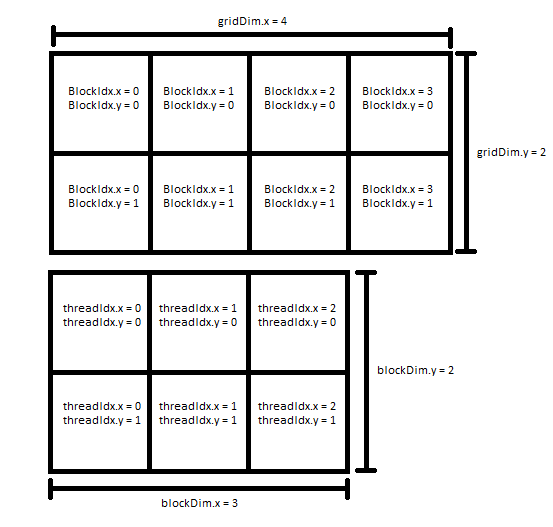
\includegraphics[width=\linewidth]{figures/gridExampleTransparant.png}}
	\caption{Example of a grid composition and block composition.}
	\label{fig1}
\end{figure}

\section{Background}

%how FW is computed
This is an optional section, as it depends on your project. In projects where a given specific knowledge is required to understand the article, you should give a brief introduction of the required concepts. In the case of genetic algorithms, you should present the basic algorithm in this section.


\section{Approach}



\section{Implementation Details}

As said before, the grid can be 1D, 2D or 3D. Our approach was to use 1D, since if for example we used 2D, we would have to do the square route of the number of blocks per thread and the number of blocks in the grid. By doing so we would possibly be wasting some threads when both numbers are not perfect squares, by doing so then it would not be archived the best occupancy.

Since by default when using GPGPU the number of computation are enormous, then one thread per computation is something not recommended, so before the launch of the kernel we used cudaOccupancyMaxPotentialBlockSize to determine the number of threads per block and number of blocks in the grid, after that we calculated the number of positions each thread would be responsible of calculating. By doing so, we would not be adding the overhead of the scheduling of each thread that would happen if there were more threads than those the GPU could run simultaneously without scheduling them.
That number would be the determined the following way:
\newline\newline
\centerline{workPerThread =$\frac{graph\_size^2}{blocksInGrid*threadsPerBlock}$}
\newline\newline
If the total positions in the matrix is not a multiple of the total number of threads launch then it should be incremented by one the value of workPerThread so that it covers the possible loss of integer division.

%falar da cena do D(i, j)

\begin{lstlisting}[language=C++, caption=Implementation Basics]
	#define EDGE_COST(graph, GRAPH_SIZE, a, b) graph[a * GRAPH_SIZE + b]
	#define D(a, b) EDGE_COST(output, GRAPH_SIZE, a, b)
\end{lstlisting}

\section{Versions}
\subsection{Sequential CPU}
In order to demonstrate the effectiveness of the usage of GPGPUs in the processing 
of some problems we started by implementing our problem in the CPU so we could use the results as a reference point to our others solutions.
%nao sei se devia por este paragrafo abaixo

This solution will only use one thread of the CPU as the purpose of this paper is to demonstrate the impact of the improvements that can be made while using a GPGPU.
%The graph we will be using for the Floyd-Warshall problem will be a two dimensional graph, in another words, a 2D grid.
With that in mind, we implemented 3 nested loops where each will start at 0 and will iterate the number of times corresponding to the size of the graph.
The second and third cycle will correspond to the X and Y coordinates, respectively, 
while the first cycle will match an intermediate point for which the shortest path will be computed.
%nao sei se meto esta ultima parte.
Inside the last cycle we will compare the direct distance of X to Y with the addition of the distances of X to K and K to Y, in case the latter is smaller the distance of X to Y is updated with the value of the addition.
Below it is possible to see our implementation:

\begin{lstlisting}[language=C++, caption=Sequential CPU]
void floyd_warshall_cpu(const int* graph, int* output) {
	
	for (int k = 0; k < GRAPH_SIZE; k++) {
		for (int i = 0; i < GRAPH_SIZE; i++) {
			for (int j = 0; j < GRAPH_SIZE; j++) {
				if (D(i, k) + D(k, j) < D(i, j)) {
					D(i, j) = D(i, k) + D(k, j);
				}
			}
		}
	}
}
\end{lstlisting}

\subsection{Sequential GPU}
To start our learning of how to program in the GPU we will start by doing the most basic implementation possible, one thread computing the entirety of the Floyd-Warshall problem.
GPU functions work like any other CPU functions barring two simple differences. 

First, a GPU function has either the "\_\_global\_\_" or the "\_\_device\_\_" qualifier.
The "\_\_global\_\_" qualifier indicates a function that will be called by the CPU but run on the GPU and "\_\_device\_\_" is a function that is called by the GPU to be run by the GPU. 
This qualifier can also be used to initialize a global variable on the GPU.

Second, the syntax of the call of a GPU function also differs. Kernels work on a grid basis, and such, you need to indicate the grid in which your program will be working on. 
That indication is made by placing
\begin{math} <<< X, Y >>> \end{math}
after the name of your function, where X represents the number of blocks to be used and Y the number of threads to be used per block, respectively. 

Having copied our graph to the GPU memory, we call our kernel with one block and one thread per block, 
Inside our GPU function we apply the same programing logic that was applied for the sequential CPU version of the Floyd-Warshall problem. 
We create 3 nested cycles to iterate through our graph and compute our problem.

Our implementation will be the following:
\begin{lstlisting}[language=C++, caption=Sequential CUDA]
	__global__ void calculateSequencialGPU(int* output)
{
	for (int k = 0; k < GRAPH_SIZE; k++) {
		for (int i = 0; i < GRAPH_SIZE; i++) {
			for (int j = 0; j < GRAPH_SIZE; j++) {
				if (D(i, k) + D(k, j) < D(i, j)) {
					D(i, j) = D(i, k) + D(k, j);
				}
			}
		}
	}
}
\end{lstlisting}


\subsection{Parallel GPU}
Using a single thread to compute a problem on the GPU goes against it's strengths. 
Due to the low core clock speed the strength of the GPU comes from it's high thread count, being able to compute multiple values at the same time. 

When running a function parallel on the GPU each thread will run it's own instance of that same function, in other words, the implementation of the function now needs to take into consideration how we partition the work load for each thread. 
Having decided the number of threads per blocks we want to use, the most common way to split the work load is to use that number to divide the size of our problem, this way obtaining the number of blocks we are going to use to compute our problem. 

With that said, like mentioned before, that method is not ideal for the problem at hand, the GPU scheduler adds a great overhead to our computation and with the increase of the size of the graph our computation will take longer and longer, something we want to avoid. Due to the fact that the number of positions in need of computation is much greater than the number of threads available and as such, we will be using all the threads and blocks available on our GPU. 
CUDA provides tools to determine said values, the "cudaDeviceProp" being one of them.

Regarding the implementation of our function, we have to change it completely.
The kernel is now called K times by the CPU, where K goes from 0 to "GRAPH\_SIZE", 
each thread will now be attributed a "WORK\_SIZE" being the number of positions they need to compute. 
We determine where the thread is located in the graph,
If the coordinates are withing the scope of the problem they will try to compute the shortest path between X to Y, using the value of K provided by the CPU when the kernel is called, updating the value if needed. 

\begin{lstlisting}[language=C++, caption=Parallel GPU]
__global__ void calcWithoutAtomic1D(int* output, int k)
{
	int totalID = blockIdx.x * blockDim.x * WORK_SIZE + threadIdx.x * WORK_SIZE;
	int i = totalID / GRAPH_SIZE;
	int j = totalID % GRAPH_SIZE;

	int counter = 0;
	while (counter < WORK_SIZE)
	{
		if (D(i, k) + D(k, j) < D(i, j)) {
			D(i, j) = D(i, k) + D(k, j);
		}
		if ((j + 1) < GRAPH_SIZE) {
			j++;
		}else {
			i++;
			j = 0;
		}
		counter++;
	}
}
\end{lstlisting}
%In order to improve performance, to the values of X and Y are added the block dimension multiplied by the dimension of the grid. After, if the coordinates are still within the scope of the problem, the thread will compute again using the new coordinates.%compute? 
\begin{comment}
	
\subsection{Work Load}

How we partition the work load for each thread may have a big impact on the performance of our solution. Like mentioned before, the major strength of the GPU is it's high thread count so that it can compute multiple values at the same time.
During our research into the topic we came up with the following guidelines in order to optimize work load: %algo me melhor k "came up with"
\begin{enumerate}
	\item Every thread works the same amount
	\item Use the most amount of threads possible
	\item Avoid using the scheduler
	\newline
\end{enumerate}
%nao gosto deste paragrafo
1. Considering every thread follows the program counter of the warp, meaning the thread is only allowed to compute a certain line when the warp allows it.
Threads with less work load might find themselves in a situation where they must sit idle waiting for others threads to catch up.
This scenario is avoided by a correct split of the work load, making every thread in the same warp be synchronized on the computation it needs to execute.
\newline
\newline
%e deste
2. Simply put, the more threads you have available to compute your problem the more you can divide your problem. A major cavite however is to not use more threads than those that are available on the GPU. When the number of threads used is bigger than those available the GPU scheduler begins to be involved a major overhead is added to the computation cutting a lot of the performance offered by the GPU.
\newline
\newline
%ja disse k nao tou inspirado hj?
3. Like mentioned before, using the GPU scheduler adds a major overhead to the computation, so it makes sense that we try to avoid using it.
One possible workaround, on a kernel call that uses loops and the problem is bigger than the number of threads offered by the GPU, is to increment the value of the coordinates variable by the product of the dimension of the block by the dimension of the grid. Doing this will allows us to reuse certain threads without having to rely on the GPU scheduler.
\newline
\newline
To show the importance of using a correct work load we will implement another solution to the Floyd-Warshall problem. First we need to decide how many blocks and threads we will be using, being both in a 2D grid. For the threads you should use the number that makes most sense considering your system, in our case that number is 8. Regarding the number of blocks we decided to use the squared root of the number of blocks allowed per multiprocessor times the number of multiprocessors present on our GPU. We then determined how much positions each thread would need to compute and send that value with our kernel call.

We determine the coordinates like previous implementations with the difference that to that number we multiply the number of positions each thread will need to compute. %fazemos isso pk....
Then we create two \textit{for} cycles that go from those coordinates to that number plus the number of positions the thread will need to compute. If the coordinates are within the scope of the problem the thread will then compute.
\end{comment}


\subsection{Synchronization}

CUDA offers it's users some forms of synchronization, allowing it's users to have a barrier on theirs implementations.
The most common forms of synchronization is using \_\_syncthreads(), which blocks the thread till all threads within the same block call it, and using Atomic variables. Atomic variables have the benefit of offering GPU wide synchronization but usage of such variables is very slow, making them only useful on certain scenarios. It is also possible to use an array where each position represents one block, where each block will increment its value and only advances when all the positions in the array are true (that is, with the value 1), but to use that the whole block should be synchronized with \_\_syncthreads() as said earlier.

Considering the Floyd-Warshall only has one barrier point, we can use synchronization to reduce the number of kernel calls to just one.
We will be using the same implementation used on the previous iteration of our solution, but slightly modifying it so it uses synchronization.
Like mentioned before atomic operations carry an heavy performance cost, so that was not the approach used, the next paragraphs will explained the solution used.

We'll start by allocating memory using cudaMalloc on the host side, for an array of integers where each position will be used only by one thread per block, that is, each block will have its own index in the array. By doing that we avoid the overhead of doing atomic operations because since each block will have its own position in the array and only one thread per block will change its value, there are no conflicts in tha manipulation of the value. The array pointer should be passed through the parameters of the kernel call and freed at the end.

Since now we will only be calling the kernel once every thread must now store it's own variable K, which will be iterated by 1 every computing cycle.  At the end of the computing cycle the first thread per block (threadIdx.x == 0) will change its value in the syncArray to 1 and then checking if all the values in that array are set to 1, if so then it shall proceed. It is important to check that before starting each iteration of K, the corresponding syncArray value will be changed now to 0.
We will be using \_\_syncthreads() so that the other threads await for the threads in each block which are responsible for the block synchronization.


\begin{lstlisting}[language=C++, caption=CUDA Example with memory improvements]
__global__ void calcWithAtomic1D(int* output, int* syncGrid)
{
	int totalID = blockIdx.x * blockDim.x * WORK_SIZE + threadIdx.x * WORK_SIZE;
	int i, j, counter, barrier, k = 0;

	while(k < GRAPH_SIZE){
		i = totalID / GRAPH_SIZE;
		j = totalID % GRAPH_SIZE;
		counter = 0;
		syncGrid[blockIdx.x] = 0;
		while (counter < WORK_SIZE)
		{
			if (D(i,k) + D(k, j) < D(i, j)) {
				D(i, j) = D(i,k) + D(k, j);
			}
			if (j + 1 < GRAPH_SIZE) {
				j++;
			}else {
				i++;
				j = 0;
			}
			counter++;
		}
		k++;

		if (threadIdx.x == 0) {
			syncGrid[blockIdx.x] = 1;
			do{
				barrier = 0;
				for(int i = 0; i < gridDim.x; i++){
					barrier += syncGrid[i];
				}
			}while(barrier != gridDim.x);
		
		}
		__syncthreads();
	}
}
\end{lstlisting}

\subsection{Memory improvements}
Shared memory is a type of memory located on-chip, meaning it is much faster then global memory. In fact shared memory latency is roughly 
100x lower than uncached global memory latency (provided that there are no bank conflicts between the threads). It is allocated per 
thread block, so all threads in the block have access to the same shared memory. The size of memory that can be used is limited, it depends on the GPU used, so when using it be aware of the GPU limitations.

Each thread has a local storage which is on-chip as the shared memory, but it is even faster due to being implemented as registers with spill over into L1 cache. This type of memory should be used every time it is possible, as the shared memory, it is even more limited.

Considering that, it should always be taken into advantage the usage of both registry and shared memory. The registry variables are created when defining new variables inside of the kernel implementation, the shared memory are the variables that are declared also inside of the kernel but with \_\_shared\_\_.

The following implementation follows the logic explained in a previous subsection, but now using registry memory to save D(i,k) that will be used multiple times, this way we avoid multiple reads from the global memory saving some time in each thread execution resulting in a better performance of the GPU kernel.

\begin{lstlisting}[language=C++, caption=CUDA Example with memory improvements]
__global__ void calcWithAtomic1DMem(int* output, int* syncGrid)
{
	int totalID = blockIdx.x * blockDim.x * WORK_SIZE + threadIdx.x * WORK_SIZE;
	int i, j , counter, k = 0, verifier, D_ik;

	while(k < GRAPH_SIZE){
		i = totalID / GRAPH_SIZE;
		j = totalID % GRAPH_SIZE;
		counter = 0;
		D_ik = D(i,k);
		syncGrid[blockIdx.x] = 0;
		while (counter < WORK_SIZE)
		{
			if (D_ik + D(k, j) < D(i, j)) {
				D(i, j) = D_ik + D(k, j);
			}
			if (j + 1 < GRAPH_SIZE) {
				j++;
			}else {
				i += ((i+1)< GRAPH_SIZE);
				j = 0;
				D_ik = D(i,k);
			}
			counter++;
		}
		k++;

		if (threadIdx.x == 0) {
			syncGrid[blockIdx.x] = 1;
			do{
				verifier = 0;
				for(int i = 0; i < gridDim.x; i++){
					verifier += syncGrid[i];
				}
			}while(verifier != gridDim.x);		
		}
		__syncthreads();
	}
}
\end{lstlisting}

In this implementation as we said, the logic is the same as the previous versions, but now taking some advantage of the fact that as it can be seen, the D(i,k) position of the matrix is repeatably read in global memory but rarely changes so we can copy it to the registry memory to reduce the overhead of reading global memory. We have to be sure that the registry memory is updated every time the i index changes so as the k value. This small change can improve significantly the performance of the kernel, even more as we increase the graph size. Depending of the problem we can take even more advantage of memory usage, this approach is only to show how the usage of shared and registry memory can have a significant improvement in performance of GPGPU.

\section{Evaluation}

\subsection{Experimental Setup}

%To be decided

\subsection{Results}

To show the results and effectiveness of our solutions we ran two sets of tests:
\begin{itemize}
	\item We ran both sequential versions with the graph size at 1000, in order to show the weakness of the GPU in single threaded tasks.
	\item We ran all our implementations, minus the sequential GPU, in order to show the impact of our improvements made on the computation of our problem.
\end{itemize}

\begin{comment}
	

In this section you should present the results. Do not forget to explain where the data came from. 

You should include (ideally vectorial) plots, with a descriptive caption. Make sure all the plots (Like Figure~\ref{fig1} are well identified and axis and metrics are defined.

\begin{figure}[htbp]
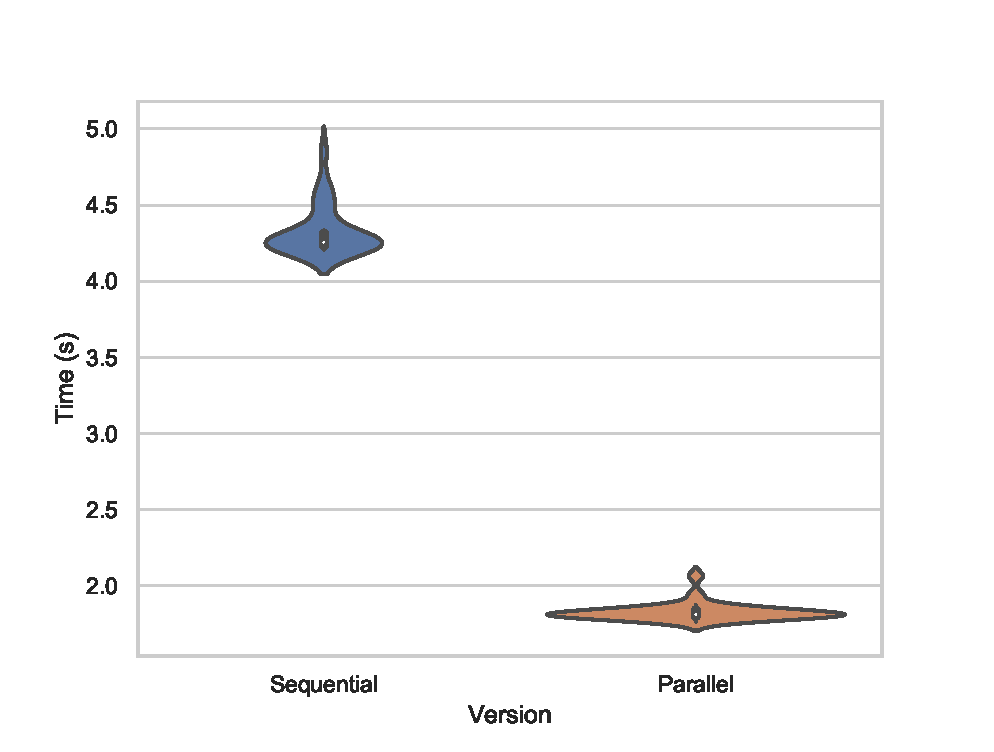
\includegraphics[width=\textwidth]{code/performance.eps}
\caption{Comparison of the performance of sequential and parallel versions of the algorithm.} \label{fig1}
\end{figure}
\end{comment}

\subsection{Discussion}



\begin{comment}
Here you should discuss the results on a high level. For instance, based on our results, the parallelization of the merge-sort is relevant as no other parallel work occurs at the same time, and the complexity $O(N log(N))$ can have a large impact when the number of individuals is high.
\end{comment}

\section{Related Work}

This section can be either the second one, or the second-to-last. In the case where knowledge of other competing works is required, it could come before. But if you are confident on what you did, it should appear at the end, where you can compare existing works against yours. An example is below:

Chu and Beasley proposed a Genetic Algorithm for the Multidimensional Knapsack Problem \cite{DBLP:journals/heuristics/ChuB98}. This work introduces a heuristic as a repair operator. Our work makes no optimization with regards to the problem domain, making it more generic and supporting other problems.

\begin{comment}

When using BibTeX references, I suggest using DBLP\footnote{\url{https://dblp.org}}, leaving Google Scholar as a backup, since DBLP has more correct and detailed information about research papers.

\end{comment}
\section{Conclusions}

Here you should resume the major conclusions taken from discussion. Ideally, these should align with the objectives introduced in the introduction.


You should also list the future work, i. e., tasks and challenges that were outside your scope, but are relevant.

\section*{Acknowledgements}

First Author wrote the part of the program implemented the phasers. Second Author implemented the MergeSort in parallel. 

Both authors wrote this paper, with First Author focusing on the introduction, related work and conclusions while the Second Author focused on approach and evaluation.

Each author spent around 30 hours on this project.

\bibliographystyle{splncs04}
\bibliography{bibliography}

\section{Ease of Use}

\subsection{Maintaining the Integrity of the Specifications}

The IEEEtran class file is used to format your paper and style the text. All margins, 
column widths, line spaces, and text fonts are prescribed; please do not 
alter them. You may note peculiarities. For example, the head margin
measures proportionately more than is customary. This measurement 
and others are deliberate, using specifications that anticipate your paper 
as one part of the entire proceedings, and not as an independent document. 
Please do not revise any of the current designations.

\section{Prepare Your Paper Before Styling}
Before you begin to format your paper, first write and save the content as a 
separate text file. Complete all content and organizational editing before 
formatting. Please note sections \ref{AA}--\ref{SCM} below for more information on 
proofreading, spelling and grammar.

Keep your text and graphic files separate until after the text has been 
formatted and styled. Do not number text heads---{\LaTeX} will do that 
for you.

\subsection{Abbreviations and Acronyms}\label{AA}
Define abbreviations and acronyms the first time they are used in the text, 
even after they have been defined in the abstract. Abbreviations such as 
IEEE, SI, MKS, CGS, ac, dc, and rms do not have to be defined. Do not use 
abbreviations in the title or heads unless they are unavoidable.

\subsection{Units}
\begin{itemize}
\item Use either SI (MKS) or CGS as primary units. (SI units are encouraged.) English units may be used as secondary units (in parentheses). An exception would be the use of English units as identifiers in trade, such as ``3.5-inch disk drive''.
\item Avoid combining SI and CGS units, such as current in amperes and magnetic field in oersteds. This often leads to confusion because equations do not balance dimensionally. If you must use mixed units, clearly state the units for each quantity that you use in an equation.
\item Do not mix complete spellings and abbreviations of units: ``Wb/m\textsuperscript{2}'' or ``webers per square meter'', not ``webers/m\textsuperscript{2}''. Spell out units when they appear in text: ``. . . a few henries'', not ``. . . a few H''.
\item Use a zero before decimal points: ``0.25'', not ``.25''. Use ``cm\textsuperscript{3}'', not ``cc''.)
\end{itemize}

\subsection{Equations}
Number equations consecutively. To make your 
equations more compact, you may use the solidus (~/~), the exp function, or 
appropriate exponents. Italicize Roman symbols for quantities and variables, 
but not Greek symbols. Use a long dash rather than a hyphen for a minus 
sign. Punctuate equations with commas or periods when they are part of a 
sentence, as in:
\begin{equation}
a+b=\gamma\label{eq}
\end{equation}

Be sure that the 
symbols in your equation have been defined before or immediately following 
the equation. Use ``\eqref{eq}'', not ``Eq.~\eqref{eq}'' or ``equation \eqref{eq}'', except at 
the beginning of a sentence: ``Equation \eqref{eq} is . . .''

\subsection{\LaTeX-Specific Advice}

Please use ``soft'' (e.g., \verb|\eqref{Eq}|) cross references instead
of ``hard'' references (e.g., \verb|(1)|). That will make it possible
to combine sections, add equations, or change the order of figures or
citations without having to go through the file line by line.

Please don't use the \verb|{eqnarray}| equation environment. Use
\verb|{align}| or \verb|{IEEEeqnarray}| instead. The \verb|{eqnarray}|
environment leaves unsightly spaces around relation symbols.

Please note that the \verb|{subequations}| environment in {\LaTeX}
will increment the main equation counter even when there are no
equation numbers displayed. If you forget that, you might write an
article in which the equation numbers skip from (17) to (20), causing
the copy editors to wonder if you've discovered a new method of
counting.

{\BibTeX} does not work by magic. It doesn't get the bibliographic
data from thin air but from .bib files. If you use {\BibTeX} to produce a
bibliography you must send the .bib files. 

{\LaTeX} can't read your mind. If you assign the same label to a
subsubsection and a table, you might find that Table I has been cross
referenced as Table IV-B3. 

{\LaTeX} does not have precognitive abilities. If you put a
\verb|\label| command before the command that updates the counter it's
supposed to be using, the label will pick up the last counter to be
cross referenced instead. In particular, a \verb|\label| command
should not go before the caption of a figure or a table.

Do not use \verb|\nonumber| inside the \verb|{array}| environment. It
will not stop equation numbers inside \verb|{array}| (there won't be
any anyway) and it might stop a wanted equation number in the
surrounding equation.

\subsection{Some Common Mistakes}\label{SCM}
\begin{itemize}
\item The word ``data'' is plural, not singular.
\item The subscript for the permeability of vacuum $\mu_{0}$, and other common scientific constants, is zero with subscript formatting, not a lowercase letter ``o''.
\item In American English, commas, semicolons, periods, question and exclamation marks are located within quotation marks only when a complete thought or name is cited, such as a title or full quotation. When quotation marks are used, instead of a bold or italic typeface, to highlight a word or phrase, punctuation should appear outside of the quotation marks. A parenthetical phrase or statement at the end of a sentence is punctuated outside of the closing parenthesis (like this). (A parenthetical sentence is punctuated within the parentheses.)
\item A graph within a graph is an ``inset'', not an ``insert''. The word alternatively is preferred to the word ``alternately'' (unless you really mean something that alternates).
\item Do not use the word ``essentially'' to mean ``approximately'' or ``effectively''.
\item In your paper title, if the words ``that uses'' can accurately replace the word ``using'', capitalize the ``u''; if not, keep using lower-cased.
\item Be aware of the different meanings of the homophones ``affect'' and ``effect'', ``complement'' and ``compliment'', ``discreet'' and ``discrete'', ``principal'' and ``principle''.
\item Do not confuse ``imply'' and ``infer''.
\item The prefix ``non'' is not a word; it should be joined to the word it modifies, usually without a hyphen.
\item There is no period after the ``et'' in the Latin abbreviation ``et al.''.
\item The abbreviation ``i.e.'' means ``that is'', and the abbreviation ``e.g.'' means ``for example''.
\end{itemize}
An excellent style manual for science writers is \cite{b7}.

\subsection{Authors and Affiliations}
\textbf{The class file is designed for, but not limited to, six authors.} A 
minimum of one author is required for all conference articles. Author names 
should be listed starting from left to right and then moving down to the 
next line. This is the author sequence that will be used in future citations 
and by indexing services. Names should not be listed in columns nor group by 
affiliation. Please keep your affiliations as succinct as possible (for 
example, do not differentiate among departments of the same organization).

\subsection{Identify the Headings}
Headings, or heads, are organizational devices that guide the reader through 
your paper. There are two types: component heads and text heads.

Component heads identify the different components of your paper and are not 
topically subordinate to each other. Examples include Acknowledgments and 
References and, for these, the correct style to use is ``Heading 5''. Use 
``figure caption'' for your Figure captions, and ``table head'' for your 
table title. Run-in heads, such as ``Abstract'', will require you to apply a 
style (in this case, italic) in addition to the style provided by the drop 
down menu to differentiate the head from the text.

Text heads organize the topics on a relational, hierarchical basis. For 
example, the paper title is the primary text head because all subsequent 
material relates and elaborates on this one topic. If there are two or more 
sub-topics, the next level head (uppercase Roman numerals) should be used 
and, conversely, if there are not at least two sub-topics, then no subheads 
should be introduced.

\subsection{Figures and Tables}
\paragraph{Positioning Figures and Tables} Place figures and tables at the top and 
bottom of columns. Avoid placing them in the middle of columns. Large 
figures and tables may span across both columns. Figure captions should be 
below the figures; table heads should appear above the tables. Insert 
figures and tables after they are cited in the text. Use the abbreviation 
``Fig.~\ref{fig}'', even at the beginning of a sentence.

\begin{table}[htbp]
\caption{Table Type Styles}
\begin{center}
\begin{tabular}{|c|c|c|c|}
\hline
\textbf{Table}&\multicolumn{3}{|c|}{\textbf{Table Column Head}} \\
\cline{2-4} 
\textbf{Head} & \textbf{\textit{Table column subhead}}& \textbf{\textit{Subhead}}& \textbf{\textit{Subhead}} \\
\hline
copy& More table copy$^{\mathrm{a}}$& &  \\
\hline
\multicolumn{4}{l}{$^{\mathrm{a}}$Sample of a Table footnote.}
\end{tabular}
\label{tab1}
\end{center}
\end{table}

%\begin{figure}[htbp]
%\centerline{
\includegraphics{fig1.png}}
%\caption{Example of a figure caption.}
%\label{fig}
%\end{figure}

Figure Labels: Use 8 point Times New Roman for Figure labels. Use words 
rather than symbols or abbreviations when writing Figure axis labels to 
avoid confusing the reader. As an example, write the quantity 
``Magnetization'', or ``Magnetization, M'', not just ``M''. If including 
units in the label, present them within parentheses. Do not label axes only 
with units. In the example, write ``Magnetization (A/m)'' or ``Magnetization 
\{A[m(1)]\}'', not just ``A/m''. Do not label axes with a ratio of 
quantities and units. For example, write ``Temperature (K)'', not 
``Temperature/K''.

\section*{Acknowledgment}

The preferred spelling of the word ``acknowledgment'' in America is without 
an ``e'' after the ``g''. Avoid the stilted expression ``one of us (R. B. 
G.) thanks $\ldots$''. Instead, try ``R. B. G. thanks$\ldots$''. Put sponsor 
acknowledgments in the unnumbered footnote on the first page.

\section*{References}

Please number citations consecutively within brackets \cite{b1}. The 
sentence punctuation follows the bracket \cite{b2}. Refer simply to the reference 
number, as in \cite{b3}---do not use ``Ref. \cite{b3}'' or ``reference \cite{b3}'' except at 
the beginning of a sentence: ``Reference \cite{b3} was the first $\ldots$''

Number footnotes separately in superscripts. Place the actual footnote at 
the bottom of the column in which it was cited. Do not put footnotes in the 
abstract or reference list. Use letters for table footnotes.

Unless there are six authors or more give all authors' names; do not use 
``et al.''. Papers that have not been published, even if they have been 
submitted for publication, should be cited as ``unpublished'' \cite{b4}. Papers 
that have been accepted for publication should be cited as ``in press'' \cite{b5}. 
Capitalize only the first word in a paper title, except for proper nouns and 
element symbols.

For papers published in translation journals, please give the English 
citation first, followed by the original foreign-language citation \cite{b6}.

\begin{thebibliography}{00}
\bibitem{b1} G. Eason, B. Noble, and I. N. Sneddon, ``On certain integrals of Lipschitz-Hankel type involving products of Bessel functions,'' Phil. Trans. Roy. Soc. London, vol. A247, pp. 529--551, April 1955.
\bibitem{b2} J. Clerk Maxwell, A Treatise on Electricity and Magnetism, 3rd ed., vol. 2. Oxford: Clarendon, 1892, pp.68--73.
\bibitem{b3} I. S. Jacobs and C. P. Bean, ``Fine particles, thin films and exchange anisotropy,'' in Magnetism, vol. III, G. T. Rado and H. Suhl, Eds. New York: Academic, 1963, pp. 271--350.
\bibitem{b4} K. Elissa, ``Title of paper if known,'' unpublished.
\bibitem{b5} R. Nicole, ``Title of paper with only first word capitalized,'' J. Name Stand. Abbrev., in press.
\bibitem{b6} Y. Yorozu, M. Hirano, K. Oka, and Y. Tagawa, ``Electron spectroscopy studies on magneto-optical media and plastic substrate interface,'' IEEE Transl. J. Magn. Japan, vol. 2, pp. 740--741, August 1987 [Digests 9th Annual Conf. Magnetics Japan, p. 301, 1982].
\bibitem{b7} M. Young, The Technical Writer's Handbook. Mill Valley, CA: University Science, 1989.
\end{thebibliography}
\vspace{12pt}
\color{red}
IEEE conference templates contain guidance text for composing and formatting conference papers. Please ensure that all template text is removed from your conference paper prior to submission to the conference. Failure to remove the template text from your paper may result in your paper not being published.

\end{document}
